\documentclass[conference,a4paper]{IEEEtran}

% Escritura mejorada de fórmulas matemáticas
\usepackage{amsmath}

% Inserción de gráficos
\usepackage{graphicx}

% Escritura de pseudocódigo
\usepackage[kw]{pseudo}

% Escritura mejorada de tablas
\usepackage{booktabs}

% Escritura mejorada de citas bibliográficas
\usepackage{cite}

%Escritura mejorada para las url
\usepackage{hyperref}


% Macros traducidas
\def\contentsname{Índice general}
\def\listfigurename{Índice de figuras}
\def\listtablename{Índice de tablas}
\def\refname{Referencias}
\def\indexname{Índice alfabético}
\def\figurename{Fig.}
\def\tablename{TABLA}
\def\partname{Parte}
\def\appendixname{Apéndice}
\def\abstractname{Resumen}
% IEEE specific names
\def\IEEEkeywordsname{Palabras clave}
\def\IEEEproofname{Demostración}


\begin{document}

\title{Tu correo, legítimo o no deseado}

\author{
  \IEEEauthorblockN{Vicente Cambrón Tocados}
  \IEEEauthorblockA{
    \textit{Dpto. Ciencias de la Computación e Inteligencia Artificial}\\
    \textit{Universidad de Sevilla}\\
    Sevilla, España\\
    viccamtoc@alum.us.es, vicentect10@gmail.com}
  
  \and
  
  \IEEEauthorblockN{José Luis García Marín}
  \IEEEauthorblockA{
    \textit{Dpto. Ciencias de la Computación e Inteligencia Artificial}\\
    \textit{Universidad de Sevilla}\\
    Sevilla, España\\
    josgarma31@alum.us.es, joselugarciamarin2406@gmail.com}
}

\maketitle


% Resumen
\begin{abstract}
  El objetivo principal de este proyecto consistía en la elaboración de un filtro para correos electrónicos no deseados mediante el empleo de técnicas de procesamiento del lenguaje natural. Con dicho propósito y para el cumplimiento del mismo, se establecieron otro tipo de objetivos para los desarrolladores del proyecto como el aprendizaje de nuevas técnicas de procesamientos del lenguaje natural para la realización de dicho filtro de correos no deseados, así como técnicas para analizar y evaluar los filtros que se habían desarrollado. Dicho análisis permitiría también conocer nuevas métricas para evaluar el trabajo realizado además de conocer cuál de los filtros realizados era el que mejor clasificaba los correos como legítimos o no deseados.
  
Gracias a este proyecto, se ha conseguido obtener todos los objetivos propuestos, así como, profundizar los conocimientos sobre el lenguaje de programación, el conocimiento y la exploración de nuevas librerías y mejorar nuestras capacidades de expresión tanto en la memoria como en el código del proyecto.
\end{abstract}


% Palabras claves
\begin{IEEEkeywords}
  Inteligencia Artificial, correos-e spam, filtro anti-spam, python, TF-IDF, KNN, Bolsa de palabras, Naive Bayes, matriz de confusión, conjunto de entrenamiento, conjunto de prueba, precisión. 
\end{IEEEkeywords}


\section{Introducción}

El objetivo de la realización de este proyecto surge de la necesidad de incorporar nuevos mecanismos de filtrado a los gestores de correos electrónicos para evitar la recepción de correos Spam. Los correos basura (Spam, en inglés) también conocidos como correos no deseados o correos no solicitados hace referencia a los mensajes de correo electrónico no deseados, no solicitados o cuyo remitente se desconoce, habitualmente de tipo publicitario, que son enviados de manera masiva perjudicando de alguna o otra manera al receptor del mensaje~\cite{b1}.

El envío de este tipo de correos ha aumentado de manera exponencial en los último años debido mayormente al interés de las empresas en dar a conocer sus productos. Por este motivo, es necesario realizar filtros de correos no deseados más firmes y certeros que permitan a los gestores de correos electrónicos desechar aquellos correos no deseados para los usuarios, mejorando así su experiencia de usuario.

Actualmente, existen multitud de técnicas y métodos aplicables para la creación de estos  filtros  de correo no deseados que se requieren hoy en día. En este proyecto, nos centraremos en una rama de la inteligencia artificial en concreto, Procesamiento del Lenguaje Natural. Dentro del campo del procesamiento del lenguaje natural nos centraremos en la aproximación empírica que usan técnicas basadas en el análisis estadístico de
grandes volúmenes de texto. Es una aproximación ascendente, ya que los modelos
se construyen a partir del propio corpus de texto del que se dispone~\cite{b2}. Algunas de las técnicas que se usarán  y que se irá explicando a lo largo del artículo son KNN, Naive Bayes multinominal y modelos de bolsa de palabras. Además, también se han utilizado otro tipo de técnicas sobre las nombradas con el fin de mejorar los filtros obtenidos. 

Con el propósito de proporcionar el mejor filtro  se realizó análisis exhaustivo para conocer cuál de los filtros desarrollados era el que realizaba la clasificación entre correos legítimos y no deseados de manera más eficiente y con un mayor número de aciertos. 

Tras la utilización de todas estas técnicas se obtuvo el resultado final y objetivo de este proyecto de investigación.

\begin{figure}
  \centering
  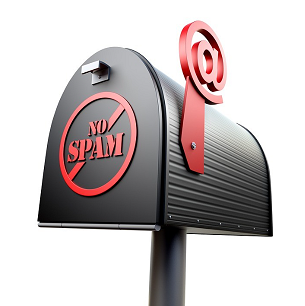
\includegraphics{spam}
  \caption{Ilustración de un buzón de un filtro Spam}
  \label{fig:spam}
\end{figure}


En los siguientes apartados de este articulo, se explicará de manera detalladas las técnicas y métodos que han sido utilizados para la construcción del filtro de correos no deseados, así como menciones a trabajos relacionados con este proyecto. Por otro lado, se añadirá la información correspondientes a los materiales y herramientas software que han sido necesarias durante las fase de desarrollo. También, se proporcionará información sobre la metodología de trabajo seguida durante la elaboración del proyecto. Además, se adjuntará  un aparatado en el que se enumeraran cuales son los resultados obtenidos y otro apartado en el que se especificarán cuales son las conclusiones obtenidas tras finalización el proyecto.



\section{Preliminares}

En esta sección, se comentará de manera breve las técnicas y métodos que han sido empleados. Por otro lado, también se hará mención a trabajos realizados por terceras personas que se asemejan al propósito de nuestro proyecto. 

En primer lugar, hablaremos sobre las técnicas y métodos empleados.


\subsection{Métodos y técnicas empleados}

Para la elaboración de los filtros, se ha empelado la tarea de clasificación de documentos, problema muy frecuentado en el procesamiento del lenguaje natural, campo de la inteligencia artificial que permite a los ordenadores entender y comprender el lenguaje humano.

Para la realización de la tarea de clasificación, se es necesario emplear dos tipos de modelos, un modelo de lenguaje y un modelo de clasificación.



\begin{itemize}
\item Modelo de lenguaje: nos permiten poder representar los documentos que se usarán tanto para representar los correos que se usarán para entrenar el algoritmo que realizará la tarea de clasificación como para representar los nuevos correos que deben ser clasificados como legítimos o no deseado.
\item Modelo de clasificación: Dado un conjunto de datos de entrenamiento, junto con las etiquetas objetivo, la clasificación determina la etiqueta de clase para un caso de prueba no etiquetado.~\cite{b4}
\end{itemize}

Durante el proyecto se ha trabajado con dos modelos de lenguaje:

\begin{itemize}
\item El modelo de bolsa de palabra que ``dado un vocabulario finito de términos V prefijado,
cada documento se representa como el vector de la cantidad de veces que ocurre cada término en el documento" ~\cite{b2}.
\item El modelo Tf-idf que es una medida numérica que expresa cuán relevante es una palabra para un documento en una colección ~\cite{b20}.
\end{itemize}

En cuanto los modelos de clasificación, modelos que nos permiten clasificar los correos entrantes como legítimos o no deseados, hay que destacar la utilización de dos tipos de estos modelos.

\begin{itemize}
\item El primero de ellos es el modelo de clasificación Naive Bayes multinominal, ``un clasificador probabilístico fundamentado en el teorema de Bayes"~\cite{b3}.
\newline

\begin{center}
$ P(A|B) =  \frac{P(A)P(B|A)}{P(B)} $\\
\end{center}

\item Él otro de los modelos que clasificación que se han empleado el modelo KNN (K Nearest Neighbors), que se consiste en buscar los k documentos más cercanos al documento a clasificar para a partir de ellos poder clasificar el nuevo documento como las clase predominante de los k documentos más cercanos ~\ref{fig:knn}. Dicho modelo ha sido utilizado para varios k, es decir, se ha probado la precisión del algoritmo para un conjunto de k vecinos diferentes. Además, los k que han sido escogido han sido siempre números impares con el objetivo de evitar los empates entre las clases a clasificar.
\end{itemize}


\begin{figure}
  \centering
  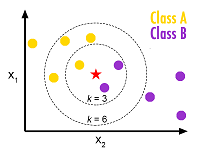
\includegraphics[scale=0.25]{knn}
  \caption{Ejemplo de una clasificación realzada mediante el modelo KNN}
  \label{fig:knn}
\end{figure}

Por otro lado, hay que destacar que se han aplicado una serie de técnicas a los modelos mencionados anteriormente con el fin de intentar mejorar estos. Las técnicas utilizadas son las siguientes:
                          
\begin{itemize}
\item Eliminación de ruido: conjunto de tareas de normalización de texto específico que a menudo tienen lugar antes de la tokenización. Algunas tareas de eliminación de ruido son:
\begin{itemize}
\item Eliminar encabezados de archivos de texto, pies de página
\item Eliminar HTML, XML, etc. marcado y metadatos
\item Extraer datos valiosos de otros formatos, como JSON 
~\cite{b8}
\end{itemize} 

\item Tokenización: es un paso que divide cadenas de texto más largas en piezas más pequeñas o tokens. Los trozos de texto más grandes pueden ser convertidos en oraciones, las oraciones pueden ser tokenizadas en palabras, etc. El procesamiento adicional generalmente se realiza después de que una pieza de texto ha sido apropiadamente concatenada. La tokenización también se conoce como segmentación de texto o análisis léxico. A veces la segmentación se usa para referirse al desglose de un gran trozo de texto en partes más grandes que las palabras (por ejemplo, párrafos u oraciones), mientras que la tokenización se reserva para el proceso de desglose que se produce exclusivamente en palabras~\cite{b9}.

\item Normalización: se refiere a una serie de tareas relacionadas destinadas a poner todo el texto en igualdad de condiciones: convirtiendo todo el texto en el mismo caso (superior o inferior), eliminando la puntuación, convirtiendo los números a sus equivalentes de palabras, y así sucesivamente. La normalización pone todas las palabras en pie de igualdad, y permite que el procesamiento proceda de manera uniforme~\cite{b10}.
\end{itemize}                                                         
                                                           
\newpage                                                           


\subsection{Trabajo Relacionado}




Hoy en día, todos los gestores de correo electrónico ofrecen una funcionalidad de filtrado de correos no deseados. En este apartado del artículo haremos mención a algunos proyectos software en los que se desarrollaron filtros anti-Spam que se usan en la actualidad.

En primer lugar, empezaremos hablando de MailWasher Free, un programa claro que funciona con todos los programas de correo electrónico. MailWasher filtra sus mensajes de correo antes de que se descarguen en su computadora (o dispositivo móvil). Verá una vista previa del correo y puede marcar los mensajes y eliminarlos antes de recuperarlos. Actualmente, se encuntra disponible para Windows, Android y MacOS y dispone de una versión gratuita para una cuenta de correo electrónico, versión de pago para varias cuentas.  ~\cite{b5}. 


Por otro lado, SPAMfighter es un filtro de spam para Outlook, Outlook Express, Windows Mail, Thunderbird y Windows Live Mail. Se produce después de que el desarrollador de software se asoció con Microsoft para crear el filtro antispam "más fuerte, seguro y efectivo" del mercado. Esencialmente, SPAMfighter bloqueará el spam de su bandeja de entrada. Si, por casualidad, aún recibe un correo electrónico no deseado, se le insta a informarlo. Esto ayudará a eliminarlo de los buzones de todos los demás miembros de la comunidad con solo un clic. En general, SPAMfighter proporciona funciones fáciles de usar y está comprobado que obtiene resultados. Disponible en dos versiones diferentes, SPAMfighter Standard y SPAMfighter PRO, la tecnología de bloqueo de spam del programa es galardonada y lo ayudará a limpiar su bandeja de entrada de inmediato ~\cite{b6}.



En último lugar, hablaremos de SpamSieve, una aplicación disponible solamente para macOS, que funciona como complemento a tu gestor de correo, y que filtra de manera inteligente todo el spam que podría llegar a tu inbox después de haberse saltado los clásicos filtros incluidos por defecto en los diferentes servidores de los servicios de correo que existen. SpamSieve puede ayudarte en este proceso gracias a su filtrado bayesiano, el cual mueve los correos que detecte que no son deseados a la carpeta de Spam. Es importante destacar esa parte de su funcionamiento ya que muchos usuarios sienten miedo a poder perder algo importante al instalar está clase de filtros, pero al simplemente mover los correos y no eliminarlos por completo, puedes estar seguro de poder recuperar un falso positivo. Además SpamSieve aprende con el tiempo, así que gracias a su potencial y un mínimo de entrenamiento por tu parte, con el tiempo podrás decirle adiós al spam prácticamente para siempre~\cite{b7}.



\section{Materiales y Herramientas}

En esta sección, nos centraremos en el lenguaje de programación utilizado para el desarrollo del código y de las librerías que han sido usadas para la implementación de dicho código.

En primer lugar, comenzaremos hablando del lenguaje de programación escogido para la realización del proyecto. La inteligencia artificial en general, y el machine learning en particular, está creciendo a un ritmo vertiginoso. El mercado necesita un número cada vez más grande de programadores capaces de aportar soluciones rápidas y funcionales, y una de las mejores formas de conseguirlo es a través de Python~\cite{b11} ~\ref{fig:python}. 

\begin{figure}
  \centering
  
\includegraphics[scale=0.25]{python}
  \caption{Logo de Python}
  \label{fig:python}
\end{figure} 



Algunas de la ventajas que nos proporciona la utilización de este lenguaje de programación son:

\begin{itemize}
\item Sencillez y facilidad de aprendizaje
\item Es open source
\item Abarca a una gran comunidad
\item Ofrece multitud de librerías
\item Versatilidad y flexibilidad
\item Excelente representación de los datos
\end{itemize}
~\cite{b11}
\\




A continuación, se nombrarán y se añadirá una breve explicación de las librería de Python ~\ref{fig:librerias} que han sido utilizadas durante el desarrollo del proyecto. 


\begin{itemize}
\item Scikit-learn es una biblioteca para aprendizaje automático de software libre. Incluye varios algoritmos de clasificación, regresión y análisis de grupos entre los cuales están máquinas de vectores de soporte, bosques aleatorios, Gradient boosting, K-means y DBSCAN. Está diseñada para interoperar con las bibliotecas numéricas y científicas NumPy y SciPy~\cite{b12}.

\item  NumPy es una biblioteca para el lenguaje de programación Python que da soporte para crear vectores y matrices grandes multidimensionales, junto con una gran colección de funciones matemáticas de alto nivel para operar con ellas~\cite{b13}.

\item OS proporciona una forma portátil de utilizar la funcionalidad dependiente del sistema operativo~\cite{b14}.

\item Email es una biblioteca para administrar mensajes de correo electrónico. No está diseñado específicamente para realizar ningún envío de mensajes de correo electrónico a SMTP (RFC 2821), NNTP u otros servidores; esas son funciones de módulos como smtplib y nntplib~\cite{b15}.

\item Re proporciona operaciones de coincidencia de expresiones reales similares a las que se encuentran en Perl~\cite{b16}.

\item Collections  implementa tipos de datos de contenedores especializados que proporcionan alternativas a los contenedores, dictados, listas, conjuntos y tuplas integrados de propósito general de Python~\cite{b17}.

\item Pickle implementa protocolos binarios para serializar y desserializar una estructura de objetos Python. "Pickling" es el proceso por el cual una jerarquía de objetos Python se convierte en un flujo de bytes, y "unpickling" es la operación inversa, mediante la cual un flujo de bytes se convierte de nuevo en una jerarquía de objetos~\cite{b18}.

\item Bs4 utilizada para analizar documentos HTML (incluyendo los que tienen un marcado incorrecto). Esta biblioteca crea un árbol con todos los elementos del documento y puede ser utilizado para extraer información~\cite{b19}.

\item Math proporciona acceso a las funciones matemáticas definidas por el estándar C. ~\cite{b21}

\item Pathlib ofrece clases que representan rutas de sistema de archivos con semántica apropiada para diferentes sistemas operativos~\cite{b22}

\item Matplotlib es una biblioteca para la generación de gráficos a partir de datos contenidos en listas o arrays en el lenguaje de programación Python y su extensión matemática NumPy.  ~\cite{b23}

\item Unicodedata proporciona acceso a la base de datos de caracteres Unicode (UCD) que define las propiedades de caracteres para todos los caracteres Unicode~\cite{b24}.

\item Nltk es un conjunto de bibliotecas y programas para el procesamiento del lenguaje natural (PLN) simbólico y estadísticos para el lenguaje de programación Python. NLTK incluye demostraciones gráficas y datos de muestra~\cite{b25}

\item Inflect proporcionan inflexiones plurales, inflexiones de sustantivos singulares, selección "a"/"an" para palabras en inglés y manipulación de números como palabras~\cite{b26}.

\item Contractions es una biblioteca de Python para expandir y crear contracciones comunes en inglés en el texto. Esto es muy útil para la reducción de la dimensionalidad al normalizar el texto antes de generar vectores de palabras o caracteres. Realiza la contracción mediante reglas de reemplazo simples de las contracciones inglesas comúnmente utilizadas. La expansión, por otro lado, no es tan simple como requiere conocimiento contextual para elegir las palabras de reemplazo correctas.~\cite{b27}

\item Split-folders es una biblioteca de Python que se encarga de dividir carpetas con archivos (por ejemplo, imágenes) en carpetas de entrenamiento, validación y prueba (conjunto de datos). ~\cite{b29}


\end{itemize}



\begin{figure}
  \centering
  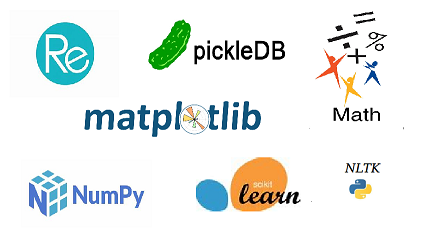
\includegraphics{librerias}
  \caption{Ejemplo de librerias de Python}
  \label{fig:librerias}
\end{figure}


\section{Metodología}

En este apartado se va a detallar cuál ha sido la metodología de trabajo seguida durante el proyecto. 


\subsection{Conjunto de entrenamiento y conjunto de prueba}
En primer lugar, se partió de un conjunto de correos que ya habían sido clasificados como legítimos o no deseados previamente. Para la creación del los filtros de correo no deseados se decidió dividir este conjunto de correo ya clasificados en dos subconjuntos. Para la realización de esta tarea se utilizó la librería split-folders. El primero de ellos se trató del conjunto de entrenamiento, el cual contendría aquellos correos que se utilizaría para que los algoritmos de clasificación. El otro de los conjuntos es el de prueba, que se utilizó para comprobar la eficacia de los algoritmos de clasificación detectando cuales de las clasificaciones habían sido verdaderos positivos, falsos positivos, verdaderos negativos y falsos negativos. La separación del conjunto inicial de correos se realizó de manera aleatoria dejando un 20\% de los correos para el subconjunto de prueba y un 80\% de los correos para el subconjunto de entrenamiento.

\subsection{Vocabulario}
Una vez separados los correos que se usaría para el entrenamiento y para las pruebas, el siguiente paso que se dió fue definir un el vocabulario de palabras, a partir del conjunto de entrenamiento, que  utilizarían los modelos de lenguaje. Para ello, el primer paso fue la extracción de los cuerpos de cada uno de los correos, tarea que pudo llevar a cabo gracias al paquete email. Posteriormente, dichos cuerpos fueron escritos y unificados que un único archivo txt que nos facilitaría el trabajo posteriormente. Debido a que los correos estaban separados en legítimos y no deseados, se obtuvieron dos de estos ficheros. A continuación, para obtener el vocabulario se leyeron los ficheros y se llevo a cabo una separación de las palabras contenidas en dicho fichero (empelando el método split de la librería re). A medida que se iban separando las palabras, estas iban siendo añadidas a un conjunto, con el objetivo de evitar palabras repetidas, y además se eliminaron aquellas palabras que contuvieran caracteres no alfanuméricos y dígitos. Una vez realizado estos pasos, se obtuvo el vocabulario completo y con el fin de evitar tener que realizar esta secuencia de acciones para poder usar el vocabulario se decidió escribir dicho vocabulario en un fichero JSON, mediante el método dump de la librería pickle, para que este pudiera ser reutilizado.



\subsection{Bolsa de Palabras y Naive Bayes Multinominal}

El primero de los filtros que se implementó fue mediante el modelo de lenguaje bolsa de palabras (Bag of Words, BoW) y el modelo de clasificación Navive Bayes multinominal. El primero de los pasos fue cargar el vocabulario que se usaría para entrenar el modelo. Para ellos se realizaban los pasos descritos previamente en la creación del vocabulario, a excepción de la existencia del fichero JSON en el que ya estaría cargado el vocabulario a utilizar y en cuyo caso se leería usando el método load de la librería pickle. Una vez conocido el vocabulario, el siguiente paso sería entrenar el modelo con el conjuntos de correos de entrenamiento. Para empezar el entrenamiento, se utilizó el método CountVectorizer, de la librería sklearn, que nos permitió contar la frecuencia de las palabras del vocabulario en los documentos, es decir, de los emails. Dicha método lo aplicamos tanto para los correos legítimos como para los no deseados del conjunto de correos de entrenamiento. El siguiente paso consistía en la obtención de los corpus que consistían en una lista de los cuerpos de los mensajes para cada clase, legítimos y no deseados. Una vez que contábamos con la frecuencia de las palabras del vocabulario y con los corpus, se llevo a cabo el entrenamiento del modelo, usando el método fit\_transform de CountVectorizer. Como resultado del entrenamiento, se obtuvo dos matrices, una para los correos legítimos y otra para los no deseados, que contenían los vectores de la frecuencia de las palabras por cada documento.

Para llevar a cabo la clasificación, se ha utilizado el clasificador Naive Bayes multinominal, el cual esta basado en la siguiente fórmula ~\eqref{eq:naive_bayes}

\begin{center}
\begin{equation}
  \label{eq:naive_bayes}
  arg \ m\acute{a}x_{c \in C} \ (P(c) \prod_{t \in 	V} P(t|c)^{n_{D,t}})
\end{equation}
\end{center}

En este punto cabe destacar que para evitar los desbordamientos numéricos las probabilidades del modelo Naive Bayes han sido calculadas mediante la siguiente fórmula~\eqref{eq:naive_bayes_desbordamiento}

\begin{center}
\begin{equation}
  \label{eq:naive_bayes_desbordamiento}
  arg \ m\acute{a}x_{c \in C} \ (log (P(c)) \ + \sum_{t \in 	V} n_{D,t} * log( P(t|c)))
\end{equation}
\end{center}

Donde C es las posibles clases en las que se puede clasificar, en este caso Legítimo y No Deseados, V hace referencia al conjunto de términos y n es la ocurrencia de un término del vocabulario en el documento.



\subsection{Modelo TF-IDF y Clasificador KNN}

El segundo y último filtro se ha implementado a través del modelo de lenguaje Tf-idf y el modelo de clasificación KNN. Como en el anterior modelo, el primer paso consistió en realizar la carga del vocabulario. El procedimiento seguido para ello exactamente el mismo que el modelo anterior. Posteriormente, se obtuvieron el corpus de entrenamiento. Difiriendo del modelo anterior, este consistía únicamente en una lista de los cuerpos de los mensajes del todo el conjunto de entrenamiento, es decir, tanto de los correos de entrenamiento legítimos como no deseados. 

Por tanto, para construir el modelo tf-idf, usamos  TfidfVectorizer de la librería sklearn. A continuación se generó el modelo con el vocabulario y se entreno dicho modelo con el corpus obtenido previamente, usando el método fit\_transform de TfidfVectorizer. El resultado de esto resulto una matriz de los vectores de obtenidos por el modelo de lenguaje tf-idf para cada documento de entrenamiento.

Para la clasificación de los correos, una vez entrenado el modelo, se genera un nuevo vector tf-idf a partir del modelo usando el método transform de TfidfVectorizer.

Por último, utilizamos el modelo de clasificación KNN, el cual asignará la clase mayoritaria de calcular las similitudes~\eqref{eq:similitud} de todos los documentos del conjuntos de entrenamientos con el nuevo correo a clasificar. 


\begin{center}
    \begin{equation}
        \label{eq:similitud}
         sim(D1,D2) = \dfrac{D1 \cdot D2}{{\|D1\| \cdot \|D2\|}} 
    \end{equation}
\end{center}

\subsection{Técnicas para mejorar los filtros }

Con el objetivo de intentar mejorar los resultados obtenidos tras la elaboración de los dos filtros explicados anteriormente, se decidió utilizar una serie de técnicas, explicadas en los aparatados anteriores del artículo. Dichas técnicas han sido utilizadas tanto en los correos de entrenamiento como en los correos de prueba, influyendo también en la creación del vocabulario. Las técnicas que se han aplicados son: eliminación de ruido, tokenización y normalización.

En primer lugar, para llevar a cabo la eliminación de ruido se han utilizados las siguientes funciones: 

\begin{enumerate}

\item \textit{Strip\_html}: se le proporciona una cadena de texto y utilizando el método BeutifulSoup de la librería bs4 conseguimos eliminar cualquier etiqueta html contenida en los correos tanto de prueba como de entrenamiento.

\item \textit{Remove\_between\_square\_brackets}: haciendo uso de la librería Re, consigue eliminar los corchetes de las cadenas de texto de los correos.

\item \textit{Replace\_contractions}: con esta función lo que conseguimos es eliminar las contracciones del inglés, por ejemplo, pasaría de ‘You’re’ a ‘You are’. Este mapeo se hace mediante el método fix de la librería contractions.

\end{enumerate}

Todas estas funciones se agrupan en una función general que reúne todos los métodos anteriormente, a la que se le pasa una cadena de texto y se le aplica todos los filtros descritos consecutivamente.

   
Por otro lado, una vez realizada la eliminación de ruido se llevo a cabo el proceso de tokenización. Para ello, se hizo uso del método \textit{word\_tokenize} de la librería nltk, al que se le pasa una cadena de texto y esta devuelve una lista de strings. Este paso se quedó registrado en la función \textit{tokenize}.

Por último, la última técnica de mejora que se decidió utilizar fue la normalización. Para introducir esta técnica en el proyecto, se implementaron los siguientes métodos:

\begin{enumerate}

\item \textit{Remove\_non\_ascii}: esta función recibe como entrada una lista de palabras tokenizadas y haciendo uso de la librería de unicodedata nos permite eliminar de los correo aquellos caracteres que no se corresponden con el código ASCII. 

\item \textit{To\_lowercase}: recibe una lista de palabras tokenizadas y se encarga de convertir cada carácter de dicha lista de palabras en su correspondiente carácter en minúsculas.

\item \textit{Remove\_punctuation}: se le pasa una lista de palabras tokenizadas y mediante la librería re se le elimina los signos de puntuación.

\item \textit{Replace\_numbers}: recibe una lista de palabras tokenizadas y haciendo uso de la librería inflect convertimos las cadenas de caracteres compuestas solo por números, y con una longitud igual e inferior a 20, a su igual en letras en inglés.

\item \textit{Remove\_stopwords}: se le pasa una lista de palabras tokenizadas y se encarga de eliminar las palabras conocidas como ‘stopwords’. Nota: dicho conjunto de palabras esta contenido dentro de la  librería NLTK. 

\item \textit{Stem\_words}: se le proporciona una lista de palabras tokenizadas y haciendo uso de LancasterStemmer de la librería nltk reduce cada cadena de la lista a su raíz (lexema). Por ejemplo, la cadena ‘Title’ a ‘Titl’.

\item \textit{Lemmatize\_verbs}: partiendo de una lista de palabras tokenizadas y haciendo uso de WordNetLemmatizer de la librería de nltk convierte cada cadena a su lema que por convenio se acepta como representante de todas las formas flexionadas de una misma palabra. Por ejemplo, ‘goe’ (stem\_words) pasaría a ‘go’.


\end{enumerate}


Por último, hay que destacar que todas estas funciones quedan recogidas en un función a la que se le proporciona la lista de palabras tokenizadas y aplica todas las funciones mencionadas anteriormente, \textit{normalize}. 

Finanalmente \textit{denoise\_text} (eliminación de ruido), \textit{tokenize} (tokenización) y \textit{normalize} (normalización), se recogieron en una misma función, llamada \textit{improve}.


\section{Resultados}

Tras la implementación de los filtros y la introducción de las mejoras mencionadas en el en apartado anterior, se llevaron a cabo una serie de pruebas con el objetivo de valorar y ver la eficiencia y efectividad de los filtros que se habían realizados, tanto con las mejoras como si ellas. 

Para ello, el primer paso que se realizó fue el entrenar los modelos mediante el conjunto de correos de entrenamiento. Una vez entrenados dichos modelos, pusimos a prueba nuestros filtros, proporcionando a las métodos que habíamos creado el conjunto de correos de prueba que habia reservado para este estudio. 

 
Como resultado de ello, se obtuvo distintas matrices de confusión variando el valor del hiperparámetro de suavizado entre 1 y 20, en el caso de bolsa de palabras y clasificador naive bayes multinominal, y el hiperparámetro k del clasificador knn y tf-idf.

Una matriz de confusión (Confusión o Error Matrix, en inglés) es una tabla que  describe el rendimiento de un modelo supervisado de Machine Learning en los datos de prueba, donde se desconocen los verdaderos valores. Se llama así porque hace que sea fácil detectar dónde el sistema está confundiéndose dos clases.~\cite{b28}
\\

\begin{figure}[hbtp]
\centering
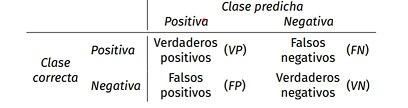
\includegraphics[scale=0.50]{matrix.jpg}
\caption{Matriz de confusión}
\end{figure}

En concreto, la clase positiva será spam y la negativa será la no\_spam (correos legítimos). Los verdaderos positivos son aquellos correos pertenecientes a la clase spam que han sido clasificados correctamente,es decir, como spam. Por otro lado, los verdaderos negativos son aquellos correos pertenecientes a la clase no\_spam que se han clasificado correctamente, como no\_spam.

Por el contrario, los falsos negativos se dan cuando un correo, perteneciente a la clase spam, se ha clasificado incorrectamente, como no\_spam. Por último, siguiendo la misma idea, los falsos positivos son aquellos correos pertenecientes a la clase no\_spam que han sido clasificados incorrectamente, como spam. 

El escenario ideal se daría cuando los falsos positivos y los falsos negativos sean ambos 0, es decir, todos los correos del prueba son clasificados correctamente.

Sin embargo, la matriz de confusión no es suficiente para poder obtener unos resultados claros para medir los filtros, aunque nos será de gran ayuda ya que la gran mayoría de las métricas de desempeño se basan en ella. Para realizar la medición de los filtros desarrollados, se ha decidido utilizar la Precisión (Accuracy) como métrica. Esta nos proporciona el porcentaje total de elementos clasificados correctamente, lo cual fue considerado como una suficiente justificación para poder elegir esta métrica y no otra porque es la medida más directa de la calidad de los clasificadores. Sin embargo, una desventaja que presenta esta métrica es que si la cantidad de elementos a evaluar de cada clase no esta balanceado, situación que no se da en nuestro caso ya que tenemos 2708 elementos pertenecientes a la clase no spam y 2374 elementos pertenecientes a la clase spam.

La precisión se calcula mediante la suma de los Verdaderos Positivos (VP) y lo Verdaderos Negativos (VN) entre el numero total de elementos (en nuestro caso emails) a clasificar, y obtenemos un valor entre 0 y 1, que mientras más alto, mejor~\eqref{eq:precision}:

\begin{center}
\begin{equation}
  \label{eq:precision}
  	Precision =  \dfrac{VP + VN}{VP + FN + FP + VN}
\end{equation}
\end{center}




Para la elección del mejor filtro se ha calculado la precisión para diferentes parámetro de los filtros. A continuación, se proporcionarán cuales han sido los mejores resultados para cada filtro.


En primer lugar, para el filtro implementado con los modelos de Bolsa de Palabras y Naive Bayes Multinominal y sin aplicar técnicas de mejoras, el mejor resultado se obtuvo con el hiperparámetro de suavizado k = 19, con una precisión aproximada del 97’80\%. A continuación, se muestra su matriz de confusión:


\begin{figure}[hbtp]
\caption{Matriz de confusión para los modelos bolsa de palabras y Naive Bayes para k = 19}
\centering
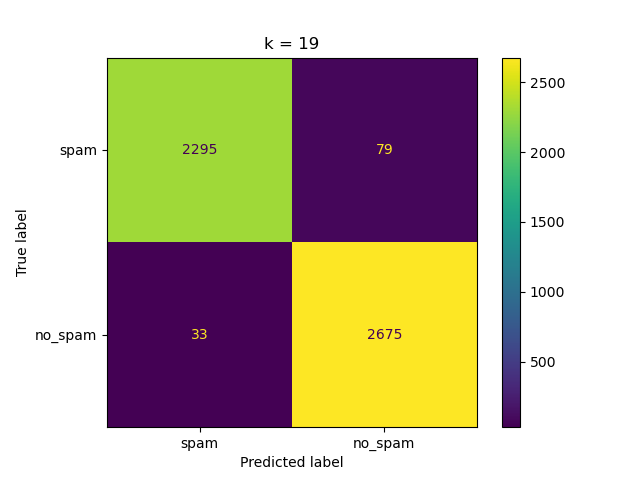
\includegraphics[scale=0.50]{bow.png}
\end{figure}

\newpage

Una vez aplicadas las técnicas de mejoras al modelo de Bolsa de Palabras su mejor resultado se obtuvo con el hiperparámetro de suavizado k = 1, con una precisión aproximada del 95’59\%. A continuación, se muestra su matriz de confusión:

\begin{figure}[hbtp]
\caption{Matriz de confusión para los modelos bolsa de palabras y Naive Bayes con las técnicas de mejora para k = 1}
\centering
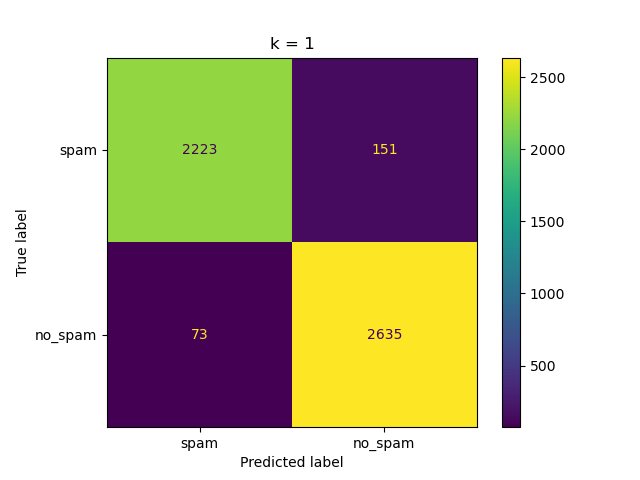
\includegraphics[scale=0.50]{bowCM.png}
\end{figure}


En el caso de TF-IDF y KNN sin aplicar técnicas de mejoras el mejor resultado se obtuvo con el parámetro k = 1 de KNN, con una precisión aproximada del 99’04\%. A continuación, se muestra su matriz de confusión:



\begin{figure}[hbtp]
\caption{Matriz de confusión para los modelosn Tf-idf y Knn para k = 1}
\centering
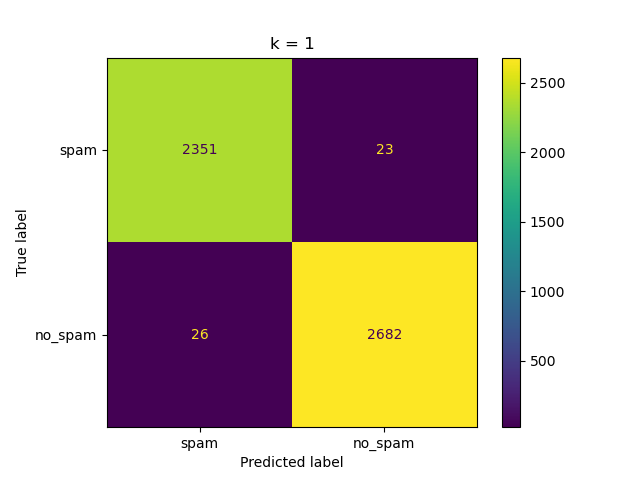
\includegraphics[scale=0.50]{tf-idf.png}
\end{figure}


Una vez aplicadas las técnicas de mejoras al modelo de TF-IDF su mejor resultado se obtuvo con el parámetro k = 1 de KNN, con una precisión aproximada del 95’79\%. A continuación, se muestra su matriz de confusión:

\begin{figure}[hbtp]
\caption{Matriz de confusión para los modelosn Tf-idf y Knn con las técnicas de mejora para k = 1}
\centering
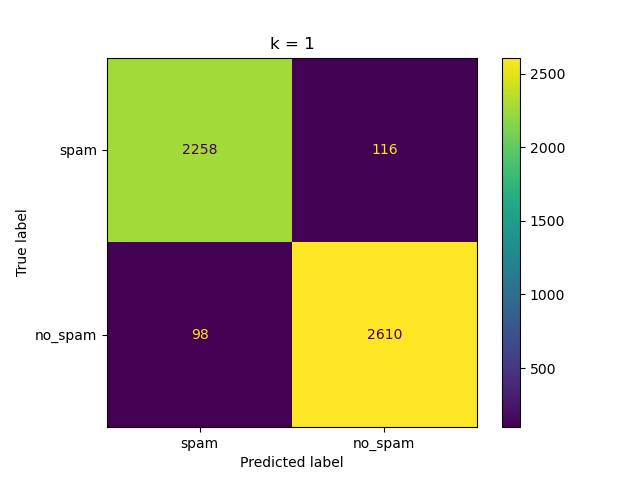
\includegraphics[scale=0.50]{tf-idfCM.png}
\end{figure}


Como se puede observar las técnicas de mejoras que hemos aplicado no han aplicado una mejora en ninguno de ambos filtros, al contrario, han empeorado la precisión de ambos. No se ha encontrado ninguna razón de porque las técnicas de mejoras empeoran ambos filtros.

Por último, se puede observar que los mejores resultados los ofrece el filtro que usa como modelo TF-IDF y clasificador KNN con valor 1 del parámetro K de KNN, con una precisión aproximada del 99’04\% sobre el conjunto de prueba. Ya que el principal objetivo de el desarrollo de este proyecto era encontrar el mejor filtro posible, se decidió establecer este ya que había sido el que mejores resultados había obtenido en la fase de prueba.





\section{Conclusiones}

Durante el proyecto, los desarrolladores involucrados en él han adquirido conocimientos a cerca de técnica utilizadas en rama de la Inteligencia Artificial, Procesamiento del Lenguaje. Gracias a él, se han conocido como implementar de manera práctica los modelos de lenguaje bolsa de palabras y tf-idf y los modelos de clasificación Naive Bayes multinominal y KNN. Por otro lado, también se han obtenido conocimientos sobre las nuevas librerías con las que se ha tenido que trabajar a los largo del desarrollo del proyecto. También, se ha estudiado la manipulación de correos electrónicos. Además de los mencionado anteriormente, se han aprendido nuevas técnicas para la mejora de modelos, así como métricas que son de gran utilidad para medir al eficiencia y eficacia de los algoritmos implementados.

En conclusión, gracias a todos los conocimientos, técnicas, métodos y modelos aprendidos se ha consigo obtener un un filtro que posee una precisión el 99\%, cumpliendo el objetivo principal del proyecto así como nos ha permitido mejorar nuestras capacidades de análisis, comprensión y expresión.

También, nos ha permitido aumentar nuestros conocimientos sobre el lenguaje de programación del proyecto, así como concer y poner en prácticas nuevos estándares de código y nuevas buenas prácticas que nos han permitido ordenar la estructura del proyecto de manera clara y legible.

Por último, como aspectos a mejorar en el futuro, cabe destacar que aunque se han aplicado técnicas para mejorar los modelos, realmente no se ha podido observar el verdadero funcionamiento de estas ya que las técnicas aplicadas en este proyecto empeoraban los resultados obtenidos. Por otro lado, también mencionar que en futuros proyectos similares, se intentaría aplicar nuevas técnicas y nuevos modelos con el objetivo de ampliar los conocimientos obtenidos.


\newpage


\begin{thebibliography}{30}
\bibitem{b1} \textsc{Correo Basura} \textit{(2022, 29 de mayo). Wikipedia, la enciclopedia libre. Fecha de consulta: 12:10, junio 7, 2022 desde} \url{https://es.wikipedia.org/wiki/Correo_basura}

\bibitem{b2} \textsc{Profesores de la asignatura Inteligencia Artificial, Dpto. de Ciencias de la Computación e Inteligencia Artificia, Universidad de Sevilla} \textit{(7/04/2022 13:15). Procesamiento del lenguaje natural. (p. 2)}

\bibitem{b4} \textsc{Moreno, I.} \textit{Introdución a la clasificación. ¿Cómo funcionan las clasificaciones y los clasificadores?} \url{https://www.statdeveloper.com/introduccion-a-la-clasificacion/}

\bibitem{b20} \textsc{Tf-idf.} \textit{(2019, 11 de diciembre). Wikipedia, La enciclopedia libre. Fecha de consulta: 18:08, junio 11, 2022 desde} \url{https://es.wikipedia.org/w/index.php?title=Tf-idf&oldid=121943707.}

 

\bibitem{b3} \textsc{Clasificador bayesiano ingenuo} \textit{2022, 22 de febrero). Wikipedia, la enciclopedia libre. Fecha de consulta: 15:40, junio 7, 2022 desde} \url{https://es.wikipedia.org/wiki/Clasificador_bayesiano_ingenuo}

\bibitem{b8} \textsc{Mayo, M} \textit{(2018, 3 de mayo). Ciencia y Datos. Preprocesamiento de datos de texto: un tutorial en Python. Eliminación de ruido} \url{https://medium.com/datos-y-ciencia/preprocesamiento-de-datos-de-texto-un-tutorial-en-python-5db5620f1767}

\bibitem{b9} \textsc{Mayo, M} \textit{(2018, 3 de mayo). Ciencia y Datos. Preprocesamiento de datos de texto: un tutorial en Python. Tokenización} \url{https://medium.com/datos-y-ciencia/preprocesamiento-de-datos-de-texto-un-tutorial-en-python-5db5620f1767}

\bibitem{b10} \textsc{Mayo, M} \textit{(2018, 3 de mayo). Ciencia y Datos. Preprocesamiento de datos de texto: un tutorial en Python. Normalización} \url{https://medium.com/datos-y-ciencia/preprocesamiento-de-datos-de-texto-un-tutorial-en-python-5db5620f1767}

\bibitem{b5} \textsc{MNI.ORG.PE} \textit{Filtros de spam. Software de filtro de spam. MailWasher Free.} \url{https://mni.org.pe/blog/filtros-de-spam/}


\bibitem{b6} \textsc{FileHippo.com }  \url{https://filehippo.com/es/download_spam-fighter/}

\bibitem{b7} \textsc{Limni} \textit{Cómo fulminar el Spam de tu email con SpamSieve. Qué es SpamSieve} \url{https://limni.net/eliminar-spam-mac-spamsieve/}



\bibitem{b11} \textsc{Structuralia} \textit{(2020, 23 de octubre). La utilidad de Python para la inteligencia artificial. Python y sus ventajas para los programadores de inteligencia artificial.} \url{https://blog.structuralia.com/python-inteligencia-artificial}

\bibitem{b12} \textsc{Scikit-learn.} \textit{(2020, 8 de noviembre). Wikipedia, La enciclopedia libre. Fecha de consulta: 11:48, junio 9, 2022 desde} \url{https://es.wikipedia.org/w/index.php?title=Scikit-learn&oldid=130746122.}

\bibitem{b13} \textsc{NumPy.} \textit{(2022, 21 de febrero). Wikipedia, La enciclopedia libre. Fecha de consulta: 11:31, junio 9, 2022 desde} \url{https://es.wikipedia.org/w/index.php?title=NumPy&oldid=141830635.}


\bibitem{b14} \textsc{Python} \textit{ 3.10.5 Documentation. The Python Standard Library. Generic Operating System Services. os — Miscellaneous operating system interfaces } \url{https://docs.python.org/3/library/os.html}


\bibitem{b15} \textsc{Python} \textit{ 3.10.5 Documentation. The Python Standard Library. Internet Data Handling. email — An email and MIME handling package } \url{https://docs.python.org/3/library/email.html?highlight=email#module-email}


\bibitem{b16} \textsc{Python} \textit{ 3.10.5 Documentation. The Python Standard Library. Text Processing Services. re — Regular expression operations. } \url{https://docs.python.org/3/library/re.html?highlight=re#module-re}

\bibitem{b17} \textsc{Python} \textit{ 3.10.5 Documentation. The Python Standard Library. Data Types. collections — Container datatypes. } \url{https://docs.python.org/3/library/collections.html?highlight=collections#module-collections}


\bibitem{b18} \textsc{Python} \textit{ 3.10.5 Documentation. The Python Standard Library. Data Persistence. pickle — Python object serialization. } \url{https://docs.python.org/3/library/pickle.html?highlight=pickle#module-pickle}


\bibitem{b19} \textsc{Beautiful Soup.} \textit{(2020, 16 de abril). Wikipedia, La enciclopedia libre. Fecha de consulta: 11:29, junio 9, 2022 desde} \url{https://es.wikipedia.org/w/index.php?title=Beautiful_Soup&oldid=125249372.}

\bibitem{b21} \textsc{Python.} \textit{3.10.5 Documentation. The Python Standard Library. Numeric and Mathematical Modules. math - Mathematical functions} \url{https://docs.python.org/3/library/math.html}

\bibitem{b22} \textsc{Python.} \textit{3.10.5 Documentation. The Python Standard Library. File and Directory Access. pathlib — Object-oriented filesystem paths} \url{https://docs.python.org/3/library/pathlib.html}

\bibitem{b23} \textsc{Matplotlib.} \textit{(2021, 11 de junio). Wikipedia, La enciclopedia libre. Fecha de consulta: 10:57, junio 24, 2022 desde} \url{https://es.wikipedia.org/w/index.php?title=Matplotlib&oldid=136252405.}


\bibitem{b24} \textsc{Python.} \textit{ 3.10.5 Documentation. The Python Standard Library. Text Processing Services. unicodedata - Unicode Database} \url{https://docs.python.org/3/library/unicodedata.html}

\bibitem{b25} \textsc{NLTK.} \textit{ (2022, 20 de febrero). Wikipedia, La enciclopedia libre. Fecha de consulta: 10:35, junio 24, 2022 desde} \url{https://es.wikipedia.org/w/index.php?title=NLTK&oldid=141812030.}

\bibitem{b26} \textsc{Python.} \textit{Inflexión 5.6.0. Descripción del proyecto. Descripción} \url{https://pypi.org/project/inflect/}

\bibitem{b27} \textsc{Python.} \textit{Pycontracciones 2.0.1. Descripción del proyecto} \url{https://pypi.org/project/pycontractions/}

\bibitem{b29} \textsc{Python.} \textit{Split-folders 0.5.1. Project description} \url{https://pypi.org/project/split-folders/}

\bibitem{b28} \textsc{Sitiobigdata.} \textit{Machine Learning: Seleccion Metricas de clasificacion. Machine Learning: Confusion Matrix} \url{https://sitiobigdata.com/2019/01/19/machine-learning-metrica-clasificacion-parte-3/}




\end{thebibliography}


\end{document}
